\section*{Anhang}
\addcontentsline{toc}{section}{Anhang}
\begin{table}
    \centering
    \caption{Netzwerk Struktur: U-Net}
    \label{tab:structure}
    \resizebox{0.45\columnwidth}{!}{
    \begin{tabular}{l c l}
        \toprule
        Layers & Output Dim. & Parameter \\
        \midrule
        Conv 2D                 & $(128, 128, 18)$ & $504$ \\       
        Dropout               & $(128, 128, 18)$ & $0  $ \\       
        Conv 2D               & $(128, 128, 18)$ & $2934  $ \\       
        Max Pooling 2D    & $(64, 64, 18)  $ & $0  $ \\       
        & & \\ 
        Conv 2D               & $(64, 64, 36)  $ & $5868  $ \\       
        Dropout             & $(64, 64, 36)  $ & $0  $ \\       
        Conv 2D               & $(64, 64, 36)  $ & $11700 $ \\       
        Max Pooling 2D  & $(32, 32, 36)  $ & $0  $ \\       
        & & \\ 
        Conv2D               & $(32, 32, 72)  $ & $23400 $ \\       
        Dropout             & $(32, 32, 72)  $ & $0  $ \\       
        Conv 2D               & $(32, 32, 72)  $ & $46728 $ \\       
        Max Pooling 2D  & $(16, 16, 72)  $ & $0  $ \\       
        & & \\ 
        Conv 2D               & $(16, 16, 144) $ & $93456 $ \\       
        Dropout             & $(16, 16, 144) $ & $0  $ \\       
        Conv 2D               & $(16, 16, 144) $ & $186768$ \\       
        Conv 2D Transpose & $(32, 32, 72)  $ & $41544 $ \\       
        Concatenate       & $(32, 32, 144) $ & $0  $ \\
        & & \\             
        Conv 2D               & $(32, 32, 72)  $ & $93384 $ \\       
        Dropout             & $(32, 32, 72)  $ & $0  $ \\       
        Conv 2D               & $(32, 32, 72)  $ & $46728 $ \\       
        Conv 2D Transpose & $(64, 64, 36)  $ & $10404 $ \\       
        Concatenate     & $(64, 64, 72)  $ & $0  $ \\                             
        & & \\             
        Conv 2D             & $(64, 64, 36)  $ & $23364 $ \\       
        Dropout             & $(64, 64, 36)  $ & $0  $ \\       
        Conv 2D              & $(64, 64, 36)  $ & $11700 $ \\       
        Conv 2D Transpose & $(128, 128, 18)$ & $2610  $ \\       
        Concatenate     & $(128, 128, 36)$ & $0  $ \\
        & & \\             
        Conv 2D             & $(128, 128, 18)$ & $5850  $ \\       
        Dropout             & $(128, 128, 18)$ & $0  $ \\       
        Conv 2D              & $(128, 128, 18)$ & $2934  $ \\       
        Conv 2D              & $(128, 128, 1) $ & $19 $ \\
        \hline
        Gesamtanzahl: & & $\SI{609895}{}$ \\
        \bottomrule
    \end{tabular}
    }
\end{table}

\begin{figure}
    \centering
    \caption{Alternative Darstellung eines U-Net zur Verdeutlich der U-förmigen Struktur. Das Level der Tiefe dieses U-Net beträgt $5$. \cite{RFB15a}}
    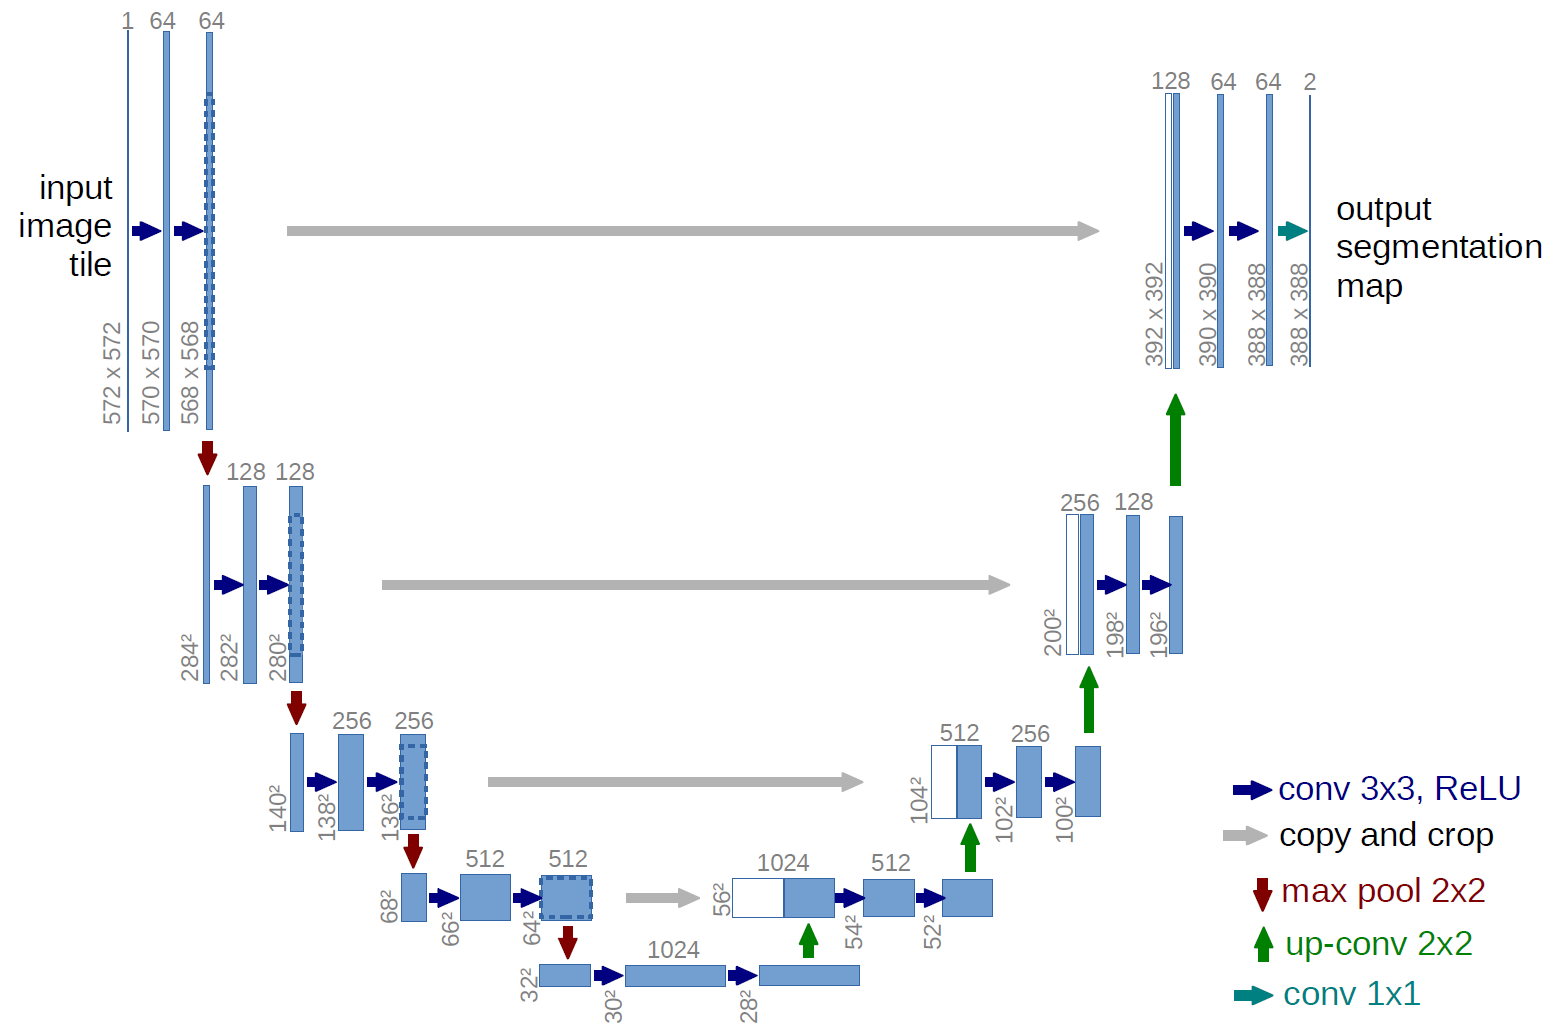
\includegraphics[width=\textwidth]{content/img/u-net-architecture.png}
\end{figure}

\begin{figure}
    \centering
    \caption{Beispielbilder für \textbf{gute} Vorhersagen des CNNs. \copyright Mapbox, \copyright OpenStreetMap}
    \label{fig:ergebnisse_gut}
    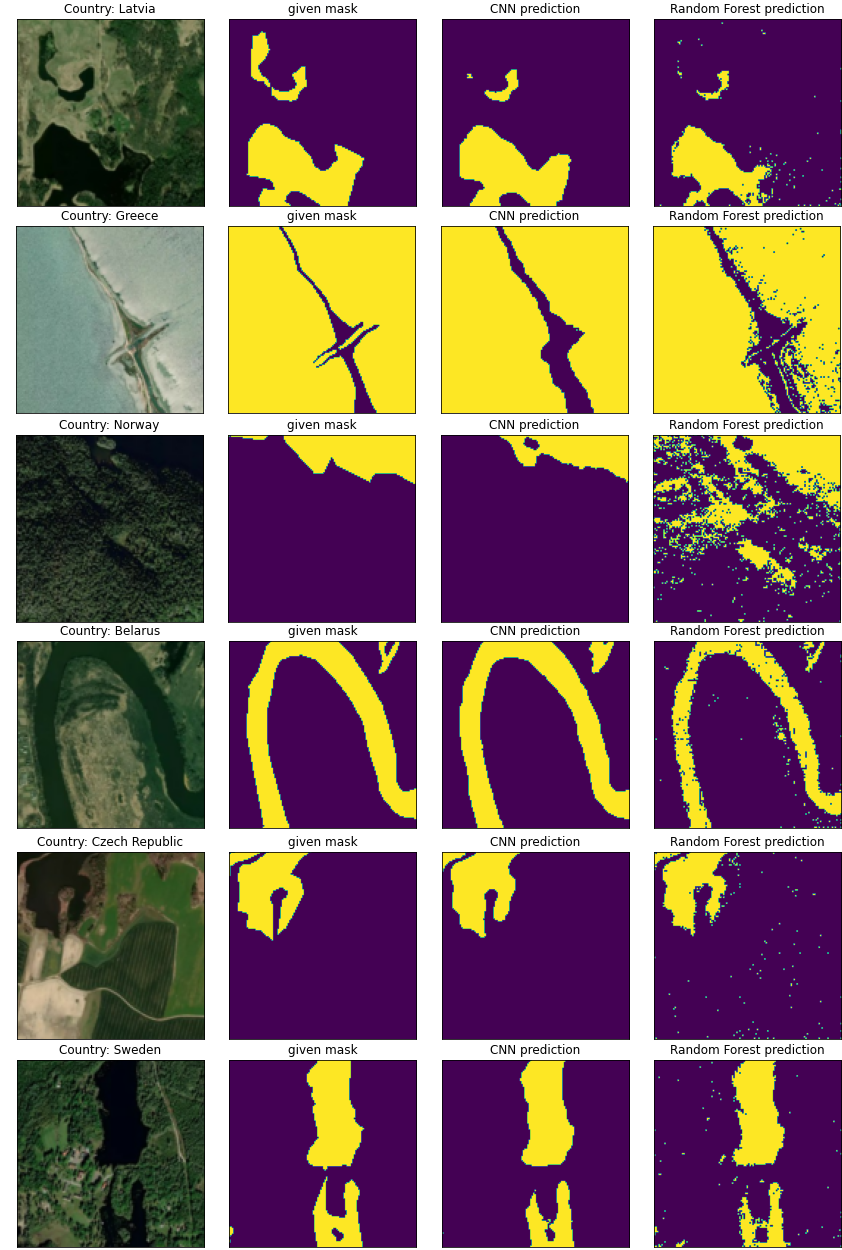
\includegraphics[width=0.95\textwidth]{content/img/ergebnisse_gut.png}
\end{figure}

\begin{figure}
    \centering
    \caption{Beispielbilder für \textbf{schlechte} Vorhersagen des CNNs. \copyright Mapbox, \copyright OpenStreetMap}
    \label{fig:ergebnisse_schlecht}
    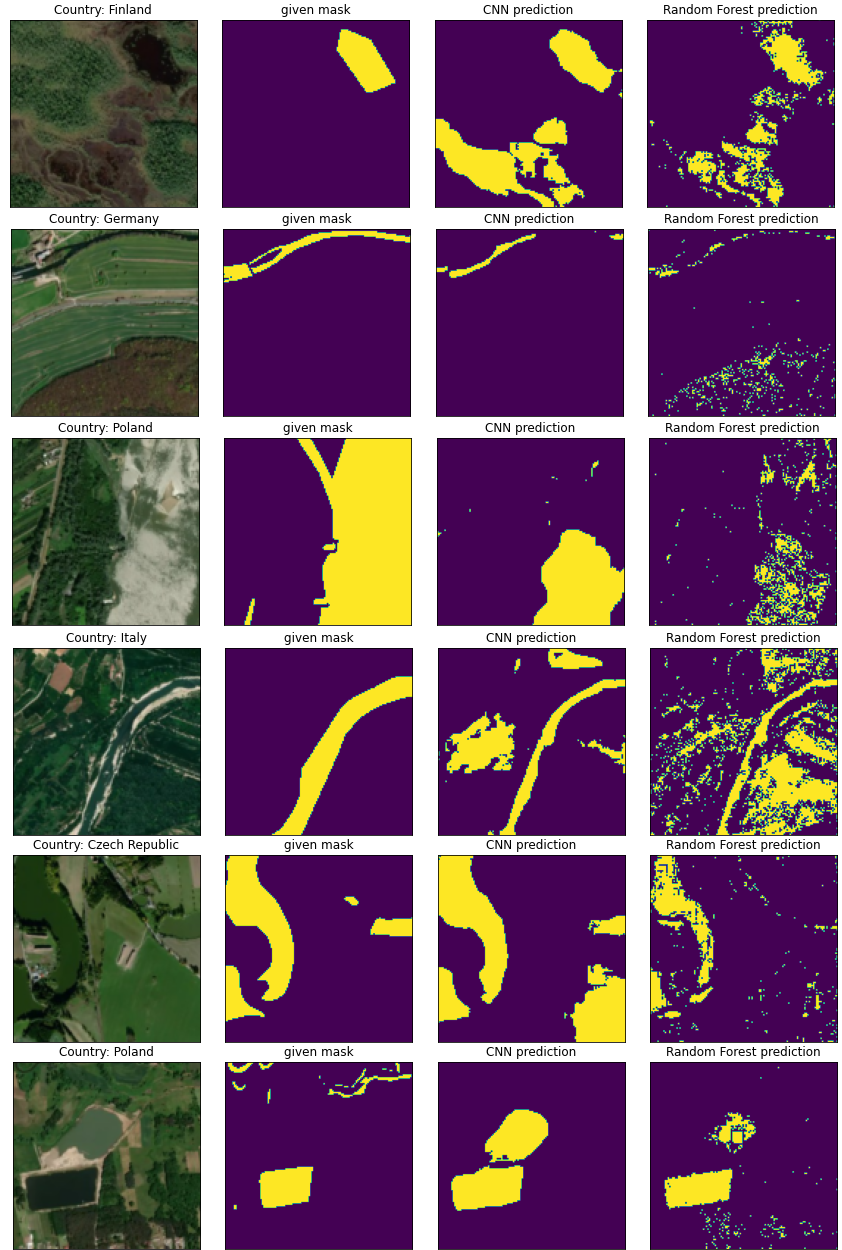
\includegraphics[width=0.95\textwidth]{content/img/ergebnisse_schlecht.png}
\end{figure}

\begin{figure}
    \centering
    \caption{Beispielbilder zur Darstellung des Gradienten und des Schwellenwerts. \copyright Mapbox, \copyright OpenStreetMap}
    \label{fig:gradient_schwellenwert}
    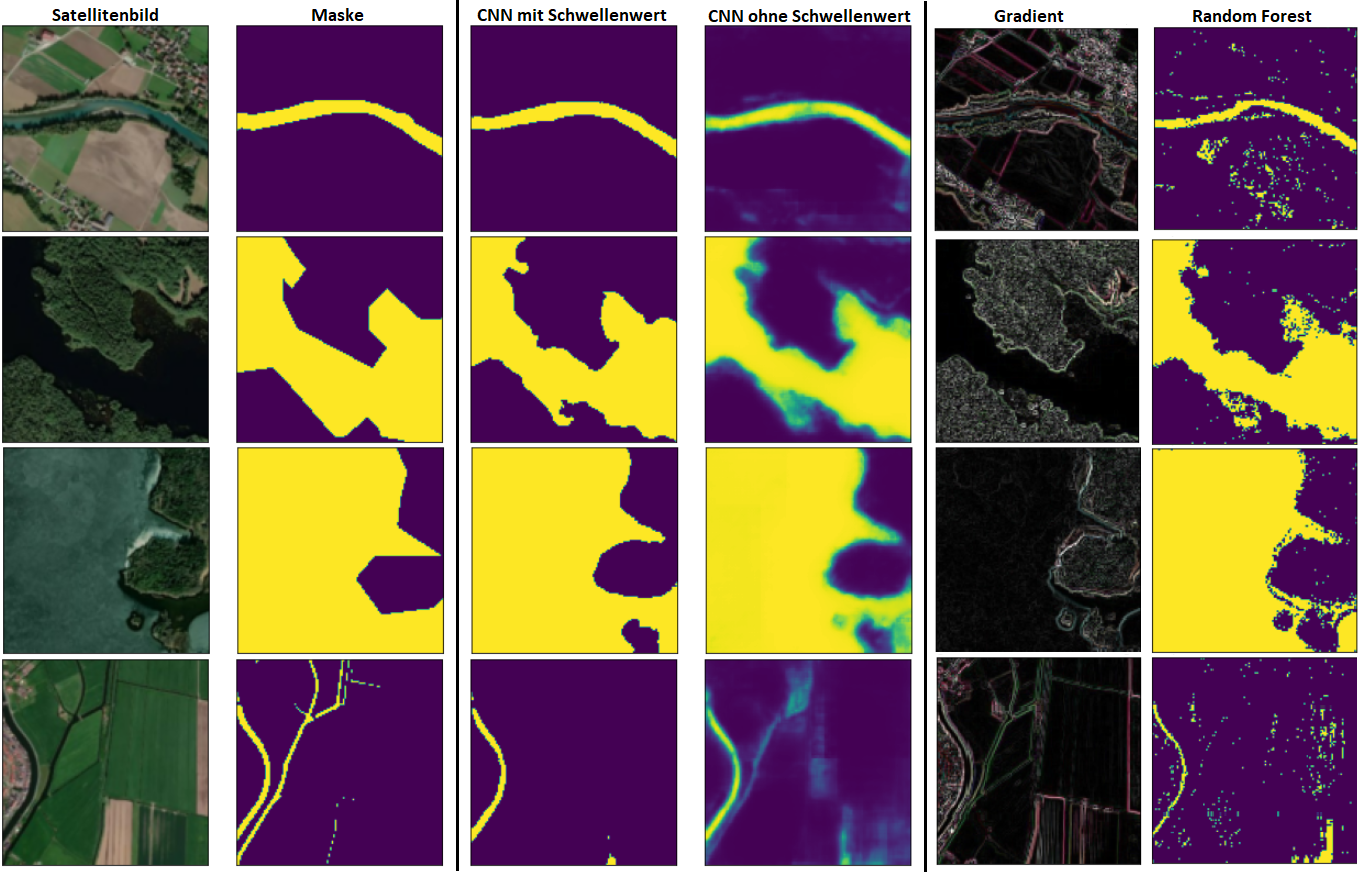
\includegraphics[width=\textwidth]{content/img/gradient_threshold.png}
\end{figure}